\documentclass[12pt]{article}
\usepackage{amsmath}
\usepackage{amsthm}
\usepackage{amssymb}
\usepackage{euscript}
\usepackage{mathrsfs}
\usepackage{bm}
\usepackage{enumitem}
\usepackage{tikz}
\usepackage{mathtools}
\usepackage{float}
\usepackage{hyperref}
\usepackage{boldline}
\usepackage{indentfirst}
\usepackage{environ}
\usepackage{courier}
\usetikzlibrary{positioning}

\renewcommand{\labelitemii}{$\vartriangleright$}
\renewcommand{\labelitemiv}{$\Join$}

\makeatletter
\newsavebox{\measure@tikzpicture}
\NewEnviron{scaletikzpicturetowidth}[1]{%
  \def\tikz@width{#1}%
  \def\tikzscale{1}\begin{lrbox}{\measure@tikzpicture}%
  \BODY
  \end{lrbox}%
  \pgfmathparse{#1/\wd\measure@tikzpicture}%
  \edef\tikzscale{\pgfmathresult}%
  \BODY
}
\makeatother

\numberwithin{equation}{section}

\hypersetup{
    colorlinks=true,
    % linkcolor=blue,
    linkcolor=[RGB]{0,0,128},
    % filecolor=[RGB]{0,0,128},
    filecolor=magenta,
    urlcolor=cyan,
    citecolor = [RGB]{128,0,128}
}

\newcommand{\myref}[2]{\hyperref[#2]{#1 \ref*{#2}}}
\newcommand{\myrefT}[1]{\hyperref[#1]{Theorem \ref*{#1}}}
\newcommand{\myrefP}[1]{\hyperref[#1]{Proposition \ref*{#1}}}
\newcommand{\myrefL}[1]{\hyperref[#1]{Lemma \ref*{#1}}}
\newcommand{\myrefD}[1]{\hyperref[#1]{Definition \ref*{#1}}}
\newcommand{\myrefn}[3]{\hyperref[#2]{#1 \ref*{#2} (#3)}}

% \input{dynkinMacros.tex}
% \input{dynkinEMacros.tex}
% \renewcommand{\qedsymbol}{}
\newcommand{\ssm}{\smallsetminus}

\newcommand{\para}[1]{\noindent\underline{#1}.}

\newcommand{\ti}{$\tau\textnormal{-invariant}$}
\newcommand{\prim}{\textnormal{Prim}_{\lambda}(\textnormal{U}(\gf))}

\newcommand{\ve}{\varepsilon}
\newcommand{\veo}{\varepsilon_1}
\newcommand{\vet}{\varepsilon_2}
\newcommand{\vei}{\varepsilon_i}
\newcommand{\vp}{\varphi}

% \newcommand{\inr}{\textnormal{In}^R}
% \newcommand{\inl}{\textnormal{In}^L}
% \newcommand{\inc}{\textnormal{In}}
% \renewcommand{\sc}{\textnormal{SC}}
% \newcommand{\re}{\textnormal{Re}}

\newcommand{\ag}{\alpha}
\newcommand{\bg}{\beta}
\newcommand{\g}{\gamma}
\newcommand{\dg}{\delta}
\newcommand{\rg}{\rho}
\newcommand{\kg}{\kappa}
\newcommand{\sg}{\sigma}
\newcommand{\tg}{\tau}
\renewcommand{\lg}{\lambda}

\renewcommand{\gg}{$\gamma \ $}
\newcommand{\ga}{$\alpha \ $}
\newcommand{\gt}{$\tau $}
\renewcommand{\(}{(\gamma)}
\newcommand{\atg}{\tilde\alpha}
\newcommand{\ags}[1]{{\ag_{#1}}}
\newcommand{\ao}{{\ag_1'}}

\newcommand{\gf}{\mathfrak g}
\newcommand{\hf}{\mathfrak h}

% needs a new name
%\newcommand{\th}[1]{{$\text{\it #1 }^{\underline{\textnormal{th}}}$}}
\renewcommand{\sf}{\mathscr F}
\newcommand{\dsf}{$\sf$}
\newcommand{\st}{\mathscr T}
% needs a new name  -- ok?
\newcommand{\so}[1]{\mathscr #1}


\newcommand{\snn}{{\mathscr S(n,n)}}
\newcommand{\smm}{{\mathscr S(M^L,M^R)}}
\renewcommand{\tan}{\mathscr T_A(n)}
\newcommand{\tn}{\mathscr T(n)}
\newcommand{\dtn}{$\tn$}
\newcommand{\tm}{\mathscr T(M)}
\newcommand{\dtm}{$\tm$}
\newcommand{\tcsn}{\mathscr T_C^S(n)}
\newcommand{\tbsn}{\mathscr T_B^S(n)}
\newcommand{\tsn}[1]{\mathscr T_#1(n)}
\newcommand{\tsm}[1]{\mathscr T_#1(M)}
\newcommand{\tnn}{\mathscr T(n,n)}
\newcommand{\tmm}{\mathscr T(M^L,M^R)}
\newcommand{\tkmm}{\mathscr T_K(M^L,M^R)}
\newcommand{\tsnn}[1]{\mathscr T_#1(n,n)}
\newcommand{\tsmm}[1]{\mathscr T_#1(M^L,M^R)}
\newcommand{\tdnn}{\mathscr T_D(n,n)}
\newcommand{\tdmm}{\mathscr T_D(M^L,M^R)}
\newcommand{\tdn}{\mathscr T_D(n)}
\newcommand{\tdm}{\mathscr T_D(M)}
\newcommand{\tcnn}{\mathscr T_C(n,n)}
\newcommand{\tcmm}{\mathscr T_C(M^L,M^R)}
\newcommand{\tcn}{\mathscr T_C(n)}
\newcommand{\tcm}{\mathscr T_C(M)}
\newcommand{\cm}{\mathscr C(M)}
\newcommand{\dm}{\mathscr D(M)}

\newcommand{\snnp}{\mathscr S'(n,n)}
\newcommand{\smmp}{\mathscr S'(M^L,M^R)}
\newcommand{\snnpp}{\mathscr S''(n,n)}
\newcommand{\smmpp}{\mathscr S''(M^L,M^R)}
\newcommand{\tnnp}{\mathscr T'(n,n)}
\newcommand{\tmmp}{\mathscr T'(M^L,M^R)}
\newcommand{\tnnpp}{\mathscr T''(n,n)}
\newcommand{\tmmpp}{\mathscr T''(M^L,M^R)}
\newcommand{\tdnnp}{\mathscr T_D'(n,n)}
\newcommand{\tdmmp}{\mathscr T_D'(M^L,M^R)}
\newcommand{\tdnnpp}{\mathscr T_D''(n,n)}
\newcommand{\tdmmpp}{\mathscr T_D''(M^L,M^R)}


\newcommand{\talb}{T_{\alpha \beta}}
\newcommand{\tai}{T_{\alpha_i,\alpha_{i+1}}}
\newcommand{\tap}{T_{\alpha_{i+1},\alpha_i}}
\newcommand{\tao}{T_{\alpha_1,\alpha_2}}
\newcommand{\tat}{T_{\alpha_2,\alpha_1}}

% new
\newcommand{\talbLeft}{T^L_{\alpha \beta}}
\newcommand{\talbRight}{T^R_{\alpha \beta}}

\newcommand{\ot}{\overline T}
\newcommand{\og}{\overline{\gamma}}

\newcommand{\sij}{{S_{ij}}}
\renewcommand{\ss}[2]{{S_{#1,#2}}}
% \def\ss#1#2{S_{#1,#2}}

\newcommand{\im}{{i-1}}
% \renewcommand{\ip}{{i+1}}
\newcommand{\ip}{{i+1}}
\newcommand{\imm}{{i-2}}
\newcommand{\ipp}{{i+2}}
\newcommand{\jm}{{j-1}}
\newcommand{\jp}{{j+1}}
\newcommand{\jmm}{{j-2}}
\newcommand{\jpp}{{j+2}}

\renewcommand{\tt}{\tau (T)}
\newcommand{\abe}{{$\{\ag,\bg\}=\{\ag_i,\ag_\ip\}$}}

\newcommand{\bt}{\mathbf T}
\newcommand{\bto}{\mathbf T_1}
\newcommand{\btt}{\mathbf T_2}
\newcommand{\obt}{\overline\bt}
\newcommand{\obto}{\overline\bt_1}
\newcommand{\obtt}{\overline\bt_2}
\newcommand{\tbt}{\tilde\bt}
\newcommand{\tbto}{\tilde\bto}
\newcommand{\tbtt}{\tilde\btt}
\newcommand{\pbt}{(\bto,\btt)}
\newcommand{\pbtp}{(\bto',\btt')}
\newcommand{\pobt}{(\obto,\obtt)}
\newcommand{\pbts}[1]{(\bto^{#1},\btt^{#1})}
\newcommand{\pobts}[1]{(\obto^{#1},\obtt^{#1})}
\newcommand{\pobtp}{(\obto',\obtt')}

\newcommand{\lo}{(\bto,\bt)}
\newcommand{\lop}{(\bto',\bt)}
\newcommand{\ls}[1]{(\bt_#1,\bt)}
\newcommand{\lsp}[1]{(\bt_#1',\bt)}
\newcommand{\ol}{(\obt_1,\obt)}

\newcommand{\be}{\mathbf E}
\newcommand{\bs}{\mathbf S}
\newcommand{\bl}{\mathbf L}
\newcommand{\br}{\mathbf R}
% \renewcommand{\op}{\bar P}
\newcommand{\op}{\bar P}
\newcommand{\pe}{P_e}

\newcommand{\oc}{\overline c}
\newcommand{\cL}{\prescript{L}{}{c}}
\newcommand{\cR}{\prescript{R}{}{c}}
\newcommand{\bc}{\mathbf c}
\newcommand{\bcL}{\prescript{L}{}{\bc}}
\newcommand{\bcR}{\prescript{R}{}{\bc}}
\newcommand{\overbc}{\overline{\mathbf c}}
\newcommand{\overcL}{\prescript{L}{}{\overline c}}
\newcommand{\overcR}{\prescript{R}{}{\overline c}}
\newcommand{\overbcL}{\prescript{L}{}{\overbc}}
\newcommand{\overbcR}{\prescript{R}{}{\overbc}}

% \newcommand{\sha}{{\textnormal{Shape}}}
\newcommand{\cs}{{c.s.p.b.}}
% \newcommand{\OC}{{\textnormal{OC}}}
% \newcommand{\OCS}{{\textnormal{OC*}}}
\newcommand{\Sf}{S_f}
\newcommand{\Sb}{S_b}
\newcommand{\nh}{n_h}
\newcommand{\nv}{n_v}
\newcommand{\rinf}{\rg_{\inf}}
\newcommand{\rsup}{\rg_{\sup}}

\newcommand{\ec}{\underset {ec}\sim}
\newcommand{\gtl}{\underset {GTL}\sim}
\newcommand{\en}{\underset {n}\sim}
\newcommand{\enm}{\underset {n-1}\sim}
\newcommand{\eqm}{\underset {m}\sim}
\newcommand{\eqmm}{\underset {m-1}\sim}
\newcommand{\ez}{\underset {0}\sim}
\newcommand{\gtr}{\underset {GTR}\sim}
\renewcommand{\gt}{\underset {GT}\sim}
\newcommand{\ngtl}{\underset {GTL}\nsim}
\newcommand{\jl}{\underset {JL}\sim}
\newcommand{\jr}{\underset {JR}\sim}
\newcommand{\kll}{\underset {KLL}\sim}
\newcommand{\klr}{\underset {KLR}\sim}

\newcommand{\fo}{F_1}
\newcommand{\ft}{F_2}
\newcommand{\fot}{\tilde\fo}
\newcommand{\ftt}{\tilde\ft}

\newcommand{\bi}{{\it b}){\it i})}
\newcommand{\bii}{{\it b}){\it ii})}

\newcommand{\sig}{\Sigma}
\newcommand{\tsl}{T_\Sigma^L}
\newcommand{\tspl}{T_{\Sigma'}^L}
\newcommand{\tssl}[1]{T_{\Sigma^#1}^L}
\newcommand{\tssbl}[1]{T_{\Sigma_#1}^L}
\newcommand{\ts}{T_\Sigma}
\newcommand{\tsp}{T_{\Sigma'}}
\newcommand{\tss}[1]{T_{\Sigma^#1}}
\newcommand{\tssb}[1]{T_{\Sigma_#1}}
\newcommand{\pin}{$\Pi\ssm\{\ag_n\}$}
\newcommand{\pc}{\phi_C}
% \newcommand{\pd}{{\phi_D}}
\newcommand{\il}{I_\lg}

\newcommand{\te}[1]{\textnormal{#1}}

\newcommand{\plainTL}{\prescript{L}{}{T}}
\newcommand{\plainTR}{\prescript{R}{}{T}}

\newcommand{\tL}{\prescript{L}{}{\bt}}
\newcommand{\tR}{\prescript{R}{}{\bt}}
\newcommand{\pairTLR}{(\tL,\tR)}
\newcommand{\pairTLRPrime}{(\tL',\tR')}
\newcommand{\pairTLRSub}[1]{(\tL_{#1},\tR_{#1})}
\newcommand{\pairTLRPrimeSub}[1]{(\tL'_{#1},\tR'_{#1})}

\newcommand{\overTL}{\prescript{L}{}{\obt}}
\newcommand{\overTR}{\prescript{R}{}{\obt}}
\newcommand{\overPairTLR}{(\overTL,\overTR)}
\newcommand{\overPairTLRPrime}{(\overTL',\overTR')}
\newcommand{\overPairTLRSub}[1]{(\overTL_{#1},\overTR_{#1})}
\newcommand{\overPairTLRPrimeSub}[1]{(\overTL'_{#1},\overTR'_{#1})}

\newcommand{\tildeTL}{\prescript{L}{}{\tbt}}
\newcommand{\tildeTR}{\prescript{R}{}{\tbt}}
\newcommand{\tildePairTLR}{(\tildeTL, \tildeTR)}
\newcommand{\pairTLRStar}{(\tL^*, \tR^*)}
\newcommand{\overPairTLRStar}{(\overTL^*, \overTR^*)}

\newcommand{\pisn}{{$\Pi^*\ssm\{\ag_n\}$}}

\newcommand{\tLSigma}{\tsl}
\newcommand{\tLSigmaSub}[1]{\tssbl#1}
\newcommand{\tDMM}{\tdmm}

\newcommand{\leftPrime}{(\tL',\tR)}
\newcommand{\leftSub}[1]{(\tL_{#1},\tR)}
\newcommand{\leftPrimeSub}[1]{(\tL_{#1}',\tR)}


\DeclareMathOperator{\Shape}{Shape}
\DeclareMathOperator{\OC}{OC}
\DeclareMathOperator{\OCS}{OC*}
% \newcommand{\inr}{\textnormal{In}^R}
% \newcommand{\inl}{\textnormal{In}^L}
% \newcommand{\inc}{\textnormal{In}}
% \renewcommand{\sc}{\textnormal{SC}}
\newcommand{\re}{\textnormal{Re}}
\DeclareMathOperator{\In}{In}
\newcommand{\inc}{\In}
\newcommand{\inL}{\In^L}
\newcommand{\inR}{\In^R}
\DeclareMathOperator{\SC}{SC}
\newcommand{\scL}{\SC^L}
\newcommand{\scR}{\SC^R}

\DeclareMathOperator{\Adj}{Adj}
\newcommand{\oeta}{\overline{\eta}}

\newcommand{\preL}[1]{\prescript{L}{}{#1}}

\newcommand{\makeBox}[2] {
  \newsavebox{#1}
  \begin{lrbox}{#1}{#2}\end{lrbox}
}

\tikzstyle{tableau} = [y = -1cm, every node/.style={transform shape}]

\definecolor{gridColor}{RGB}{19,83,150}
\tikzstyle{dominoStyle} = [color=black, fill=white, rounded corners = .1cm, thick]
\tikzstyle{gridLine} = [color=gridColor, thick]
\tikzstyle{dominoText} = [font=\Large, midway]
\tikzstyle{cycleLine} = [color=green, thick, >->]
\tikzstyle{closedCycleLine} = [color=green, thick]
% \tikzstyle{fixedSquareStyle} = [pattern = crosshatch doats, pattern color=gridColor,  opacity=0.2]
\tikzstyle{fixedSquareStyle} = [color=gridColor,  opacity=0.07]
\tikzstyle{tileText} = [font=\large, midway]

\newcommand{\eps}{.06}
\newcommand{\teps}{\eps * 2}

% first entry is row, starting with 1, second entry is column, third is content
\newcommand{\filledSquare}[3]{\filldraw [dominoStyle] (#2 - 1 + \eps, #1 - 1 + \eps) rectangle + (1 - \teps, 1 -\teps) node [tileText] {$#3$};}
% The fourth entry shifts vertically
\newcommand{\filledSquareShift}[4]{\filldraw [dominoStyle] (#2 - 1 + #4 + \eps, #1 - 1 + \eps) rectangle + (1 - \teps, 1 -\teps) node [tileText] {$#3$};}

\newcommand{\horizontalDomino}[3]{\filldraw [dominoStyle] (#2 - 1 + \eps, #1 - 1 + \eps) rectangle + (2 - \teps, 1 -\teps) node [dominoText] {$#3$};}
\newcommand{\verticalDomino}[3]{\filldraw [dominoStyle] (#2 - 1 + \eps,  #1 - 1 + \eps) rectangle + (1 - \teps,2 -\teps) node [dominoText] {$#3$};}

\newcommand{\horizontalDominoShift}[4]{\filldraw [dominoStyle] (#2 - 1 + #4 + \eps, #1 - 1 + \eps) rectangle + (2 - \teps, 1 -\teps) node [dominoText] {$#3$};}
\newcommand{\verticalDominoShift}[4]{\filldraw [dominoStyle] (#2 - 1 + #4 + \eps,  #1 - 1 + \eps) rectangle + (1 - \teps,2 -\teps) node [dominoText] {$#3$};}

\newcommand{\zeroSquare}[2]{\filldraw [dominoStyle] (#2 - 1 + \eps, #1 - 1 + \eps) rectangle + (1 - \teps, 1 -\teps) node [dominoText] {$0$};}
\newcommand{\zeroSquareShift}[3]{\filldraw [dominoStyle] (#2 - 1 + #3 + \eps, #1 - 1 + \eps) rectangle + (1 - \teps, 1 -\teps) node [dominoText] {$0$};}


\newcommand{\emptyBox}[2]{\filldraw [dominoStyle] (#2 - 1 + \eps, #1 - 1 + \eps) rectangle + (2 - \teps, 2 -\teps);}
\newcommand{\signedBox}[3]{
\filldraw [opacity=0] (#2 - 1 + 1, #1 - 1) rectangle + (1, 2) node [dominoText,opacity=1] {$#3$};
\filldraw [dominoStyle, fill opacity = 0] (#2 - 1 + \eps, #1 - 1 + \eps) rectangle + (2 - \teps, 2 -\teps);
}

\newcommand{\emptyBoxShift}[3]{\filldraw [dominoStyle] (#2 - 1 + #3 + \eps, #1 - 1 + \eps) rectangle + (2 - \teps, 2 -\teps);}
\newcommand{\signedBoxShift}[4]{
\filldraw [opacity=0] (#2 - 1 + 1 + #4, #1 - 1) rectangle + (1, 2) node [dominoText,opacity=1] {$#3$};
\filldraw [dominoStyle, fill opacity = 0] (#2 - 1 + #4 + \eps, #1 - 1 + \eps) rectangle + (2 - \teps, 2 -\teps);
}

% These rows and columns are zero-based
\newcommand{\horizontalGridLine}[3]{\draw [gridLine] (#1, #2) -- + (#3,0);}
\newcommand{\verticalGridLine}[2]{\draw [gridLine] (#1, 0) -- + (0,#2);}
\newcommand{\fixedSquare}[2]{\filldraw [fixedSquareStyle] (#1,#2) rectangle +(1,1);}

% This will have #1 * 2 rows and #2 *2 columns
\newcommand{\gridLines}[2] {
  \pgfmathsetmacro{\verticalEnd}{2 * #1}
  \pgfmathsetmacro{\horizontalEnd}{2 * #2}
  \foreach \vertical in {0,...,#2} {
    \pgfmathsetmacro{\var} {2 * \vertical}
    \verticalGridLine{\var}{\verticalEnd}
  }
  \foreach \horizontal in {0,...,#1} {
    \pgfmathsetmacro{\var} {2 * \horizontal}
    \horizontalGridLine{0}{\var}{\horizontalEnd}
  }
}

% This will have #1 * 2 rows and #2 *2 columns
% The vertical lines will be shifted over #3 squares
\newcommand{\gridLinesShift}[3] {
  \pgfmathsetmacro{\verticalEnd}{2 * #1}
  \pgfmathsetmacro{\horizontalEnd}{2 * #2}
  \foreach \vertical in {0,...,#2} {
    \pgfmathsetmacro{\var} {2 * \vertical + #3}
    \verticalGridLine{\var}{\verticalEnd}
  }
  \foreach \horizontal in {0,...,#1} {
    \pgfmathsetmacro{\var} {2 * \horizontal}
    \horizontalGridLine{#3}{\var}{\horizontalEnd}
  }
}

\newcommand{\fixedSquaresStart}[4]{
  \foreach \row in {#1,...,#2} {
    \foreach \column in {#3,...,#4} {
      \pgfmathsetmacro{\var}{\row + \column}
      \ifodd \var
      \else
        \fixedSquare\column\row
      \fi
    }
  }
}

\newcommand{\fixedSquares}[2]{
  \foreach \row in {0,...,#1} {
    \foreach \column in {0,...,#2} {
      \pgfmathsetmacro{\var}{\row + \column}
      \ifodd \var
        \fixedSquare\column\row
      \fi
    }
  }
}

% This has #1 * 2 rows and #2 * 2 columns
\newcommand{\fixedSquaresForGrid}[2] {
  \pgfmathsetmacro{\rowParameter}{#1 * 2 - 1}
  \pgfmathsetmacro{\columnParameter}{#2 * 2 - 1}
  \fixedSquares{\rowParameter}{\columnParameter}
}

% This has #1 * 2 rows and #2 * 2 columns
% The vertical lines will be shifted over #3 squares
\newcommand{\fixedSquaresForGridShift}[3] {
  \pgfmathsetmacro{\rowParameter}{#1 * 2 - 1}
  \pgfmathsetmacro{\columnStart}{#3}
  \pgfmathsetmacro{\columnEnd}{#2 * 2 - 1 + #3}
  \fixedSquaresStart{0}{\rowParameter}{\columnStart}{\columnEnd}
}

\newcommand{\fixedSquaresStartAlt}[4]{
  \foreach \row in {#1,...,#2} {
    \foreach \column in {#3,...,#4} {
      \pgfmathsetmacro{\var}{\row + \column + 1}
      \ifodd \var
      \else
        \fixedSquare\column\row
      \fi
    }
  }
}

% This has #1 * 2 rows and #2 * 2 columns
% The vertical lines will be shifted over #3 squares
\newcommand{\fixedSquaresForGridShiftAlt}[3] {
  \pgfmathsetmacro{\rowParameter}{#1 * 2 - 1}
  \pgfmathsetmacro{\columnStart}{#3}
  \pgfmathsetmacro{\columnEnd}{#2 * 2 - 1 + #3}
  \fixedSquaresStartAlt{0}{\rowParameter}{\columnStart}{\columnEnd}
}


% This will have #1 rows and #2 columns
\newcommand{\typeAGridLines}[2] {
  \foreach \vertical in {0,...,#2} {
    \verticalGridLine{\vertical}{#1}
  }
  \foreach \horizontal in {0,...,#1} {
    \horizontalGridLine{0}{\horizontal}{#2}
  }
}

% This will have #1 rows and #2 columns
% The vertical lines will be shifted over #3 squares
\newcommand{\typeAGridLinesShift}[3] {
  \foreach \vertical in {0,...,#2} {
    \pgfmathsetmacro{\var} {\vertical + #3}
    \verticalGridLine{\var}{#1}
  }
  \foreach \horizontal in {0,...,#1} {
    \horizontalGridLine{#3}{\horizontal}{#2}
  }
}

\newcommand{\euscr}{\EuScript}

\newcommand{\upLineLabel}[4]{\draw[-, thick, #1] (#2.north) -- node[right]{$#4$} (#3.south);}
\newcommand{\sideLine}[3]{\draw[-, thick, dashdotted, #1] (#2.east) -- (#3.west);}

\newcommand{\bdot}{\begin{tikzpicture}[close]
  \filldraw (0, 0) circle (3pt);
\end{tikzpicture}
}
\newcommand{\upLineLabelPos}[5]{\draw[-, thick, #1] (#2.north) -- node[#5]{$#4$} (#3.south);}
\newcommand{\sideLineStyle}[4]{\draw[-, thick, #1, #2] (#3.east) -- (#4.west);}

\DeclarePairedDelimiter\abs{\lvert}{\rvert}

\newcommand{\upperLabel}[1]{\node[draw, brown, text = black, inner sep = .3cm] at (current bounding box.north) {\Large{#1}};}

\tikzstyle{dominoMaybeStyle} = [color=blue, dashed, fill=white, rounded corners = .1cm, thick]

\newcommand{\horizontalDominoMaybe}[3]{\filldraw [dominoMaybeStyle] (#2 - 1 + \eps, #1 - 1 + \eps) rectangle + (2 - \teps, 1 -\teps) node [dominoText] {$#3$};}
\newcommand{\verticalDominoMaybe}[3]{\filldraw [dominoMaybeStyle] (#2 - 1 + \eps,  #1 - 1 + \eps) rectangle + (1 - \teps,2 -\teps) node [dominoText] {$#3$};}
\newcommand{\horizontalDominoMaybeShift}[4]{\filldraw [dominoMaybeStyle] (#2 - 1 + #4 + \eps, #1 - 1 + \eps) rectangle + (2 - \teps, 1 -\teps) node [dominoText] {$#3$};}
\newcommand{\verticalDominoMaybeShift}[4]{\filldraw [dominoMaybeStyle] (#2 - 1 + #4 + \eps,  #1 - 1 + \eps) rectangle + (1 - \teps,2 -\teps) node [dominoText] {$#3$};}

\newcommand{\greenCircle}[2]{\filldraw[green] (#2 - .5, #1 - .5) circle (.2cm);}

\setlist[itemize]{listparindent=1.25em, parsep=0pt}

\begin{document}
  Finally, our last situation is grid position $W$.
  As before, we'll assume the sign which we are adding is $+$.
  We're looking to add at position $(x, y)$.
  To be looking to add at grid positon $W$, there must be an unboxed cycle directly to the left.
  There must also be a sign in the row above (TODO, why?  We've asked this question before.)

  Here is a quick overview.
  If the leftmost sign in the row above is negative, we are good to go.
  We can add here as a horizontal domino, extending the unboxed cycle.
  If not, we need to look at the domino directly to the left, which we'll call the adjacent domino.
  Our cases will depend on whether this domino is horizontal or vertical.

  Now, we'll do the cases in the code.
  We'll refer to the domino just above, in the $(x - 1, y)$ fixed square, as the pair domino.
  Note, the pair domino is the cycle top.
  \begin{itemize}
    \item Here the adjacent domino is horizontal and the leftmost sign in the row above is $+$.
    Then we can't add here.
    We go to the next row.
    \begin{figure}[H]
      \centering
      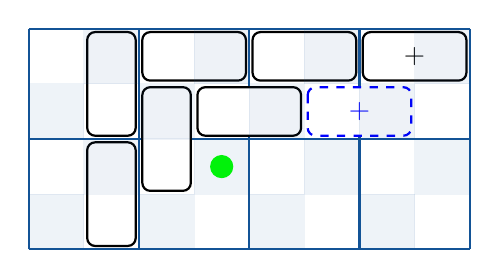
\begin{tikzpicture}[tableau, scale = .7]
        \gridLines{2}{4}
        \verticalDomino{1}{2}{}
        \horizontalDomino{1}{3}{}
        \horizontalDomino{1}{5}{}
        \horizontalDomino{1}{7}{+}
        \verticalDomino{2}{3}{}
        \verticalDomino{3}{2}{}
        \horizontalDomino{2}{4}{}
        \horizontalDominoMaybe{2}{6}{+}
        \greenCircle{3}{4}
        \fixedSquaresForGrid{2}{4}
      \end{tikzpicture}
      \item
    \end{figure}
    \item Here the pair domino has a $-$ sign.
    We can add here, as a horizontal domino.
    This works whether or not the adjacent domino is horizontal.
    Note, the row above has to have length at least $x + 3$, or we couldn't get here (TODO, prove this).
    (We'll illustrate with the adjacent domino vertical since that makes for smaller examples.)
    Since the pair domino has a $-$ sign and is the cycle top, the adjacent domino either has a $-$ sign or is blank.  Those are our two cases.
    \begin{itemize}
      \item If the adjacent domino has a $-$ sign, we don't have to do anything more.
      The new domino will pair with it, and legitimately extend the signs in the pairing.
      \begin{figure}[H]
        \centering
        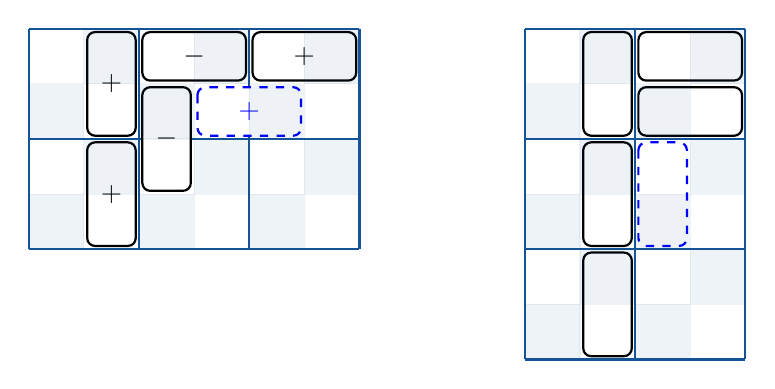
\begin{tikzpicture}[tableau, scale = .7]
          \gridLines{2}{3}
          \verticalDomino{1}{2}{+}
          \horizontalDomino{1}{3}{-}
          \horizontalDomino{1}{5}{+}
          \verticalDomino{2}{3}{-}
          \horizontalDominoMaybe{2}{4}{+}
          \verticalDomino{3}{2}{+}
          \fixedSquaresForGrid{2}{3}

          \gridLinesShift{3}{2}{9}
          \verticalDominoShift{1}{2}{}{9}
          \horizontalDominoShift{1}{3}{}{9}
          \horizontalDominoShift{2}{3}{}{9}
          \verticalDominoShift{3}{2}{ }{9}
          \verticalDominoShift{5}{2}{ }{9}
          \verticalDominoMaybeShift{3}{3}{ }{9}
          \fixedSquaresForGridShift{3}{2}{9}
        \end{tikzpicture}
      \end{figure}
      \begin{figure}[H]
        % 1+ 2- 3_-4 5+ 6+
        \centering
        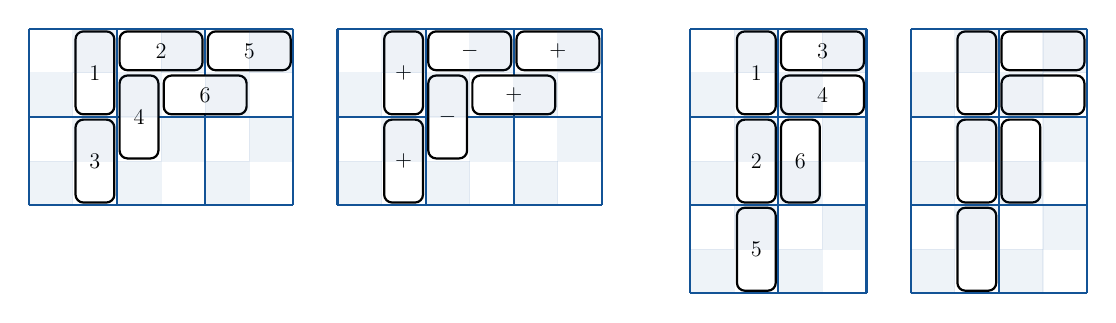
\begin{tikzpicture}[tableau, scale=.56]\gridLines{2}{3}\verticalDomino{1}{2}{1}\horizontalDomino{1}{3}{2}\verticalDomino{3}{2}{3}\verticalDomino{2}{3}{4}\horizontalDomino{1}{5}{5}\horizontalDomino{2}{4}{6}\fixedSquaresForGrid{2}{3}\gridLinesShift{2}{3}{7}\verticalDominoShift{1}{2}{+}{7}\horizontalDominoShift{1}{3}{-}{7}\verticalDominoShift{3}{2}{+}{7}\verticalDominoShift{2}{3}{-}{7}\horizontalDominoShift{1}{5}{+}{7}\horizontalDominoShift{2}{4}{+}{7}\fixedSquaresForGridShift{2}{3}{7}\gridLinesShift{3}{2}{15}\verticalDominoShift{1}{2}{1}{15}\verticalDominoShift{3}{2}{2}{15}\horizontalDominoShift{1}{3}{3}{15}\horizontalDominoShift{2}{3}{4}{15}\verticalDominoShift{5}{2}{5}{15}\verticalDominoShift{3}{3}{6}{15}\fixedSquaresForGridShift{3}{2}{15}\gridLinesShift{3}{2}{20}\verticalDominoShift{1}{2}{}{20}\verticalDominoShift{3}{2}{}{20}\horizontalDominoShift{1}{3}{}{20}\horizontalDominoShift{2}{3}{}{20}\verticalDominoShift{5}{2}{}{20}\verticalDominoShift{3}{3}{}{20}\fixedSquaresForGridShiftAlt{3}{2}{20}\end{tikzpicture}
      \end{figure}
      \item If the adjacent domino is blank, we'll have to blank the added domino and the pair domino, and put signs in the corresponding dual dominoes.
      (Note, I'm expecting that the domino to the right of the pair domino has a $+$, rather than being blank.  TODO, prove this.)
      \begin{figure}[H]
        \centering
        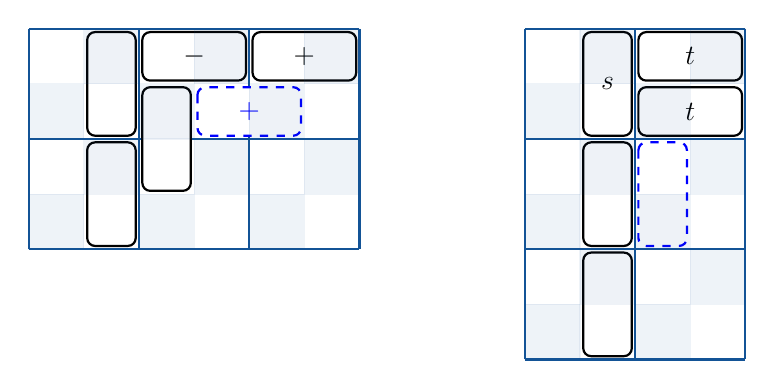
\begin{tikzpicture}[tableau, scale = .7]
          \gridLines{2}{3}
          \verticalDomino{1}{2}{}
          \horizontalDomino{1}{3}{-}
          \horizontalDomino{1}{5}{+}
          \verticalDomino{2}{3}{}
          \horizontalDominoMaybe{2}{4}{+}
          \verticalDomino{3}{2}{}
          \fixedSquaresForGrid{2}{3}

          \gridLinesShift{3}{2}{9}
          \verticalDominoShift{1}{2}{s}{9}
          \horizontalDominoShift{1}{3}{t}{9}
          \horizontalDominoShift{2}{3}{t}{9}
          \verticalDominoShift{3}{2}{}{9}
          \verticalDominoShift{5}{2}{ }{9}
          \verticalDominoMaybeShift{3}{3}{ }{9}
          \fixedSquaresForGridShift{3}{2}{9}
        \end{tikzpicture}
      \end{figure}
      goes to
      \begin{figure}[H]
        \centering
        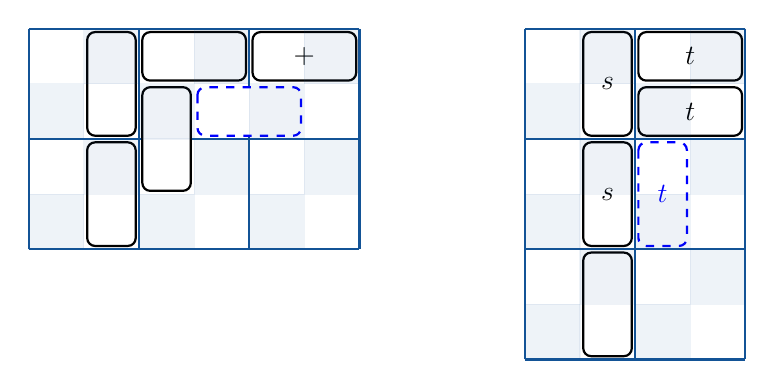
\begin{tikzpicture}[tableau, scale = .7]
          \gridLines{2}{3}
          \verticalDomino{1}{2}{}
          \horizontalDomino{1}{3}{}
          \horizontalDomino{1}{5}{+}
          \verticalDomino{2}{3}{}
          \horizontalDominoMaybe{2}{4}{}
          \verticalDomino{3}{2}{}
          \fixedSquaresForGrid{2}{3}

          \gridLinesShift{3}{2}{9}
          \verticalDominoShift{1}{2}{s}{9}
          \horizontalDominoShift{1}{3}{t}{9}
          \horizontalDominoShift{2}{3}{t}{9}
          \verticalDominoShift{3}{2}{s}{9}
          \verticalDominoShift{5}{2}{ }{9}
          \verticalDominoMaybeShift{3}{3}{t}{9}
          \fixedSquaresForGridShift{3}{2}{9}
        \end{tikzpicture}
      \end{figure}
      \begin{figure}[H]
        % 1s 2- 3t 4t 5+ 6+
        \centering
        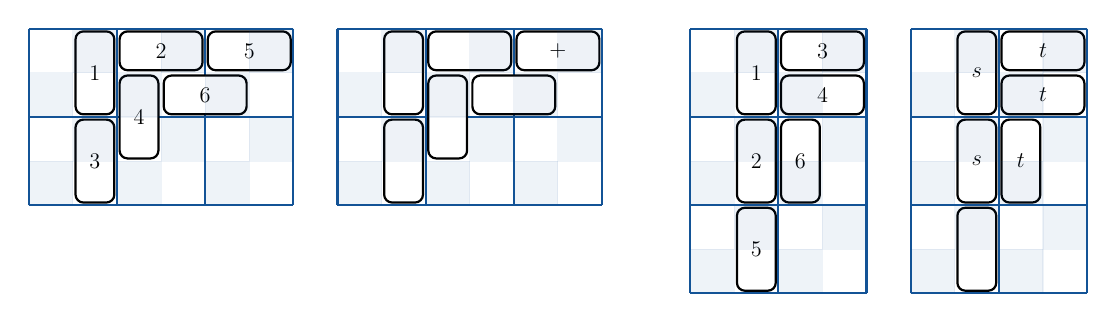
\begin{tikzpicture}[tableau, scale=.56]\gridLines{2}{3}\verticalDomino{1}{2}{1}\horizontalDomino{1}{3}{2}\verticalDomino{3}{2}{3}\verticalDomino{2}{3}{4}\horizontalDomino{1}{5}{5}\horizontalDomino{2}{4}{6}\fixedSquaresForGrid{2}{3}\gridLinesShift{2}{3}{7}\verticalDominoShift{1}{2}{}{7}\horizontalDominoShift{1}{3}{}{7}\verticalDominoShift{3}{2}{}{7}\verticalDominoShift{2}{3}{}{7}\horizontalDominoShift{1}{5}{+}{7}\horizontalDominoShift{2}{4}{}{7}\fixedSquaresForGridShift{2}{3}{7}\gridLinesShift{3}{2}{15}\verticalDominoShift{1}{2}{1}{15}\verticalDominoShift{3}{2}{2}{15}\horizontalDominoShift{1}{3}{3}{15}\horizontalDominoShift{2}{3}{4}{15}\verticalDominoShift{5}{2}{5}{15}\verticalDominoShift{3}{3}{6}{15}\fixedSquaresForGridShift{3}{2}{15}\gridLinesShift{3}{2}{20}\verticalDominoShift{1}{2}{s}{20}\verticalDominoShift{3}{2}{s}{20}\horizontalDominoShift{1}{3}{t}{20}\horizontalDominoShift{2}{3}{t}{20}\verticalDominoShift{5}{2}{}{20}\verticalDominoShift{3}{3}{t}{20}\fixedSquaresForGridShiftAlt{3}{2}{20}\end{tikzpicture}
      \end{figure}
    \end{itemize}
    \item Here the pair domino is blank and the sign in the above row is $-$
    As in the previous case, we can add here, as a horizontal domino.
    This works whether or not the adjacent domino is horizontal.
    Note, the row above has to have length at least $x + 3$, since we have the blank pair domino plus at least one signed domino to the right.
    (Again, we'll illustrate with the adjacent domino vertical since that makes for smaller examples.)

    As in the code, we'll call the domino with the $-$ sign the right domino.
    In all cases, we'll be blanking the right domino's sign (while bringing its sign to the pair domino), so we'll be putting a sign in the dual domino corresponding to the right domino.
    We'll use \texttt{prepareForSign()} on the dual side for that.

    Since the pair domino is blank, we have all three possibilities for the sign of the adjacent domino.
    Those are our three cases.
    Once we've moved the $-$ sign from the right domino to the pair domino, we have two opposite signs in the pair domino and newly-added domino.
    We can do what we like with them.
    So, we'll alter them to be compatible with the signs already in the paired cycles.
    \begin{itemize}
      \item Here the adjacent domino has a $-$ sign.
      We don't have to do anything else.
      \begin{figure}[H]
        \centering
        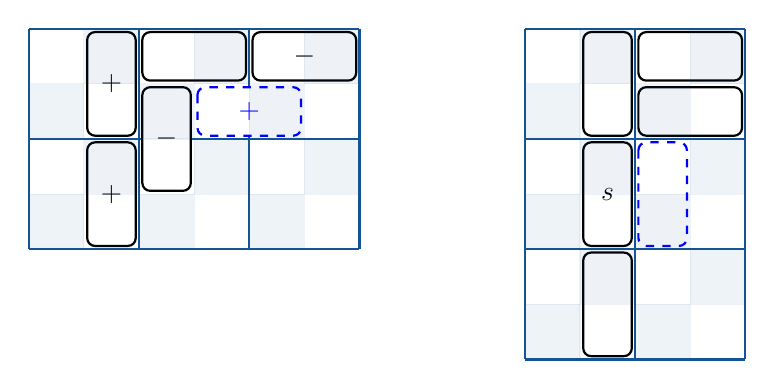
\begin{tikzpicture}[tableau, scale = .7]
          \gridLines{2}{3}
          \verticalDomino{1}{2}{+}
          \horizontalDomino{1}{3}{}
          \horizontalDomino{1}{5}{-}
          \verticalDomino{2}{3}{-}
          \horizontalDominoMaybe{2}{4}{+}
          \verticalDomino{3}{2}{+}
          \fixedSquaresForGrid{2}{3}

          \gridLinesShift{3}{2}{9}
          \verticalDominoShift{1}{2}{}{9}
          \horizontalDominoShift{1}{3}{}{9}
          \horizontalDominoShift{2}{3}{}{9}
          \verticalDominoShift{3}{2}{s}{9}
          \verticalDominoShift{5}{2}{ }{9}
          \verticalDominoMaybeShift{3}{3}{ }{9}
          \fixedSquaresForGridShift{3}{2}{9}
        \end{tikzpicture}
      \end{figure}
      goes to
      \begin{figure}[H]
        \centering
        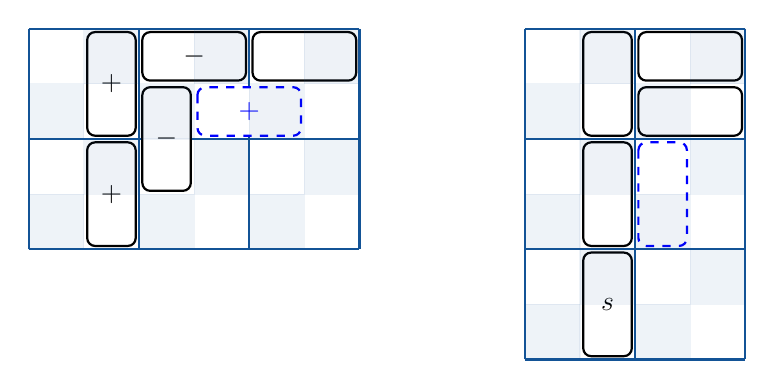
\begin{tikzpicture}[tableau, scale = .7]
          \gridLines{2}{3}
          \verticalDomino{1}{2}{+}
          \horizontalDomino{1}{3}{-}
          \horizontalDomino{1}{5}{}
          \verticalDomino{2}{3}{-}
          \horizontalDominoMaybe{2}{4}{+}
          \verticalDomino{3}{2}{+}
          \fixedSquaresForGrid{2}{3}

          \gridLinesShift{3}{2}{9}
          \verticalDominoShift{1}{2}{}{9}
          \horizontalDominoShift{1}{3}{}{9}
          \horizontalDominoShift{2}{3}{}{9}
          \verticalDominoShift{3}{2}{}{9}
          \verticalDominoShift{5}{2}{s}{9}
          \verticalDominoMaybeShift{3}{3}{ }{9}
          \fixedSquaresForGridShift{3}{2}{9}
        \end{tikzpicture}
      \end{figure}
      \begin{figure}[H]
        % 1s 2+ 3_-4 5_6
        \centering
        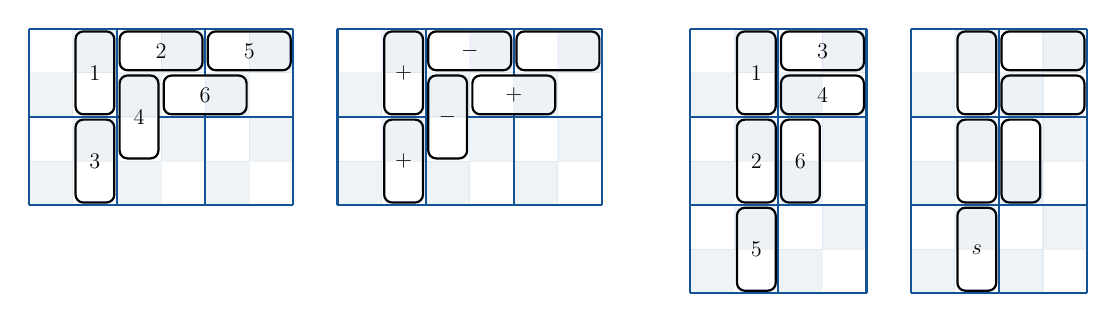
\begin{tikzpicture}[tableau, scale=.56]\gridLines{2}{3}\verticalDomino{1}{2}{1}\horizontalDomino{1}{3}{2}\verticalDomino{3}{2}{3}\verticalDomino{2}{3}{4}\horizontalDomino{1}{5}{5}\horizontalDomino{2}{4}{6}\fixedSquaresForGrid{2}{3}\gridLinesShift{2}{3}{7}\verticalDominoShift{1}{2}{+}{7}\horizontalDominoShift{1}{3}{-}{7}\verticalDominoShift{3}{2}{+}{7}\verticalDominoShift{2}{3}{-}{7}\horizontalDominoShift{1}{5}{}{7}\horizontalDominoShift{2}{4}{+}{7}\fixedSquaresForGridShift{2}{3}{7}\gridLinesShift{3}{2}{15}\verticalDominoShift{1}{2}{1}{15}\verticalDominoShift{3}{2}{2}{15}\horizontalDominoShift{1}{3}{3}{15}\horizontalDominoShift{2}{3}{4}{15}\verticalDominoShift{5}{2}{5}{15}\verticalDominoShift{3}{3}{6}{15}\fixedSquaresForGridShift{3}{2}{15}\gridLinesShift{3}{2}{20}\verticalDominoShift{1}{2}{}{20}\verticalDominoShift{3}{2}{}{20}\horizontalDominoShift{1}{3}{}{20}\horizontalDominoShift{2}{3}{}{20}\verticalDominoShift{5}{2}{s}{20}\verticalDominoShift{3}{3}{}{20}\fixedSquaresForGridShiftAlt{3}{2}{20}\end{tikzpicture}
      \end{figure}
      \item Here the adjacent domino has a $+$ sign.
      After moving the $-$ sign to the pair domino, we need to swap the signs in the pair domino and the newly-added domino, to be compatible with sign pattern already on the cycle.
      \begin{figure}[H]
        \centering
        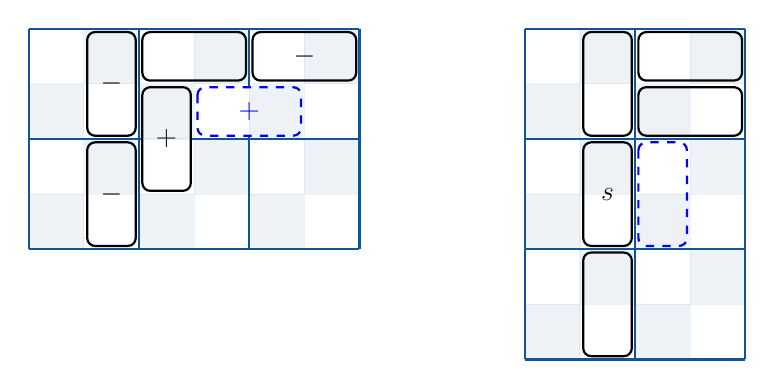
\begin{tikzpicture}[tableau, scale = .7]
          \gridLines{2}{3}
          \verticalDomino{1}{2}{-}
          \horizontalDomino{1}{3}{}
          \horizontalDomino{1}{5}{-}
          \verticalDomino{2}{3}{+}
          \horizontalDominoMaybe{2}{4}{+}
          \verticalDomino{3}{2}{-}
          \fixedSquaresForGrid{2}{3}

          \gridLinesShift{3}{2}{9}
          \verticalDominoShift{1}{2}{}{9}
          \horizontalDominoShift{1}{3}{}{9}
          \horizontalDominoShift{2}{3}{}{9}
          \verticalDominoShift{3}{2}{s}{9}
          \verticalDominoShift{5}{2}{ }{9}
          \verticalDominoMaybeShift{3}{3}{ }{9}
          \fixedSquaresForGridShift{3}{2}{9}
        \end{tikzpicture}
      \end{figure}
      goes to
      \begin{figure}[H]
        \centering
        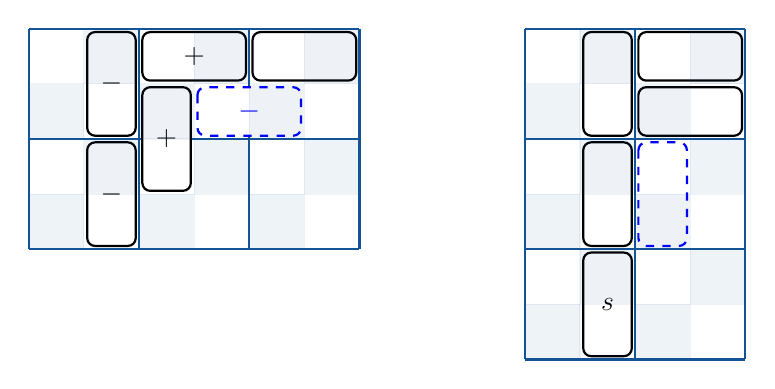
\begin{tikzpicture}[tableau, scale = .7]
          \gridLines{2}{3}
          \verticalDomino{1}{2}{-}
          \horizontalDomino{1}{3}{+}
          \horizontalDomino{1}{5}{}
          \verticalDomino{2}{3}{+}
          \horizontalDominoMaybe{2}{4}{-}
          \verticalDomino{3}{2}{-}
          \fixedSquaresForGrid{2}{3}

          \gridLinesShift{3}{2}{9}
          \verticalDominoShift{1}{2}{}{9}
          \horizontalDominoShift{1}{3}{}{9}
          \horizontalDominoShift{2}{3}{}{9}
          \verticalDominoShift{3}{2}{}{9}
          \verticalDominoShift{5}{2}{s}{9}
          \verticalDominoMaybeShift{3}{3}{ }{9}
          \fixedSquaresForGridShift{3}{2}{9}
        \end{tikzpicture}
      \end{figure}
      \begin{figure}[H]
        % 1s 2- 3_-4 5- 6+ 7+
        \centering
        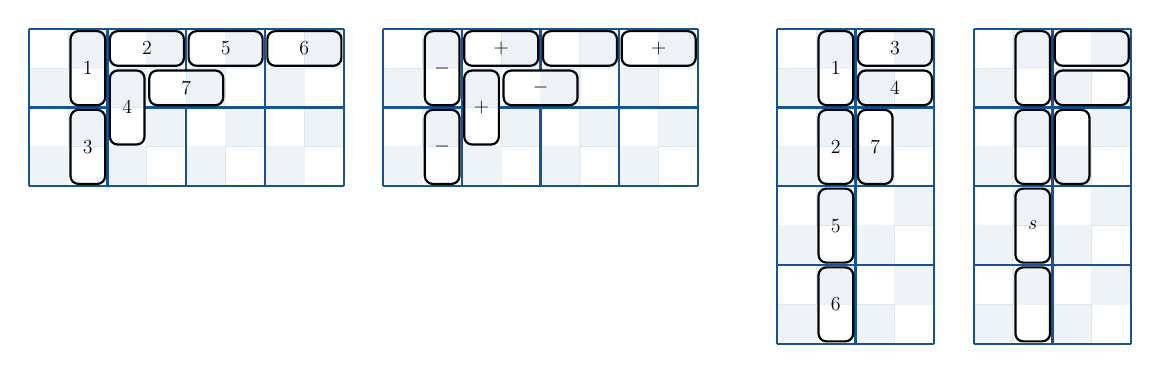
\begin{tikzpicture}[tableau, scale=.5]\gridLines{2}{4}\verticalDomino{1}{2}{1}\horizontalDomino{1}{3}{2}\verticalDomino{3}{2}{3}\verticalDomino{2}{3}{4}\horizontalDomino{1}{5}{5}\horizontalDomino{1}{7}{6}\horizontalDomino{2}{4}{7}\fixedSquaresForGrid{2}{4}\gridLinesShift{2}{4}{9}\verticalDominoShift{1}{2}{-}{9}\horizontalDominoShift{1}{3}{+}{9}\verticalDominoShift{3}{2}{-}{9}\verticalDominoShift{2}{3}{+}{9}\horizontalDominoShift{1}{5}{}{9}\horizontalDominoShift{1}{7}{+}{9}\horizontalDominoShift{2}{4}{-}{9}\fixedSquaresForGridShift{2}{4}{9}\gridLinesShift{4}{2}{19}\verticalDominoShift{1}{2}{1}{19}\verticalDominoShift{3}{2}{2}{19}\horizontalDominoShift{1}{3}{3}{19}\horizontalDominoShift{2}{3}{4}{19}\verticalDominoShift{5}{2}{5}{19}\verticalDominoShift{7}{2}{6}{19}\verticalDominoShift{3}{3}{7}{19}\fixedSquaresForGridShift{4}{2}{19}\gridLinesShift{4}{2}{24}\verticalDominoShift{1}{2}{}{24}\verticalDominoShift{3}{2}{}{24}\horizontalDominoShift{1}{3}{}{24}\horizontalDominoShift{2}{3}{}{24}\verticalDominoShift{5}{2}{s}{24}\verticalDominoShift{7}{2}{}{24}\verticalDominoShift{3}{3}{}{24}\fixedSquaresForGridShiftAlt{4}{2}{24}\end{tikzpicture}
      \end{figure}
      \item Here the adjacent domino is blank.
      After moving the $-$ sign to the pair domino, we need to blank the pair domino and the newly-added domino, and to put appropriate signs into their corresponding dominoes, so as to be compatible with sign pattern already in the cycle.
      \begin{figure}[H]
        \centering
        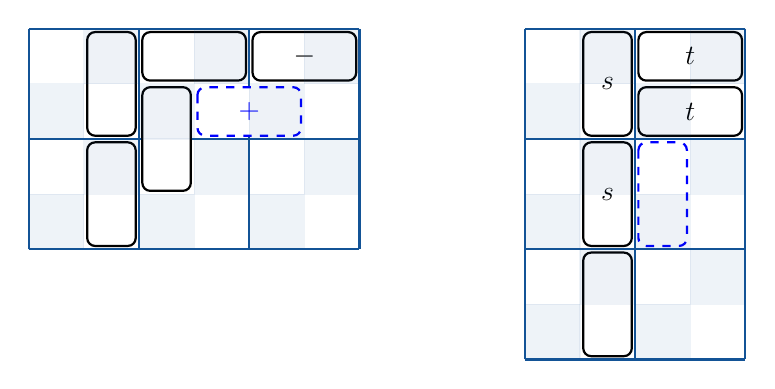
\begin{tikzpicture}[tableau, scale = .7]
          \gridLines{2}{3}
          \verticalDomino{1}{2}{}
          \horizontalDomino{1}{3}{}
          \horizontalDomino{1}{5}{-}
          \verticalDomino{2}{3}{}
          \horizontalDominoMaybe{2}{4}{+}
          \verticalDomino{3}{2}{}
          \fixedSquaresForGrid{2}{3}

          \gridLinesShift{3}{2}{9}
          \verticalDominoShift{1}{2}{s}{9}
          \horizontalDominoShift{1}{3}{t}{9}
          \horizontalDominoShift{2}{3}{t}{9}
          \verticalDominoShift{3}{2}{s}{9}
          \verticalDominoShift{5}{2}{ }{9}
          \verticalDominoMaybeShift{3}{3}{ }{9}
          \fixedSquaresForGridShift{3}{2}{9}
        \end{tikzpicture}
      \end{figure}
      goes to
      \begin{figure}[H]
        \centering
        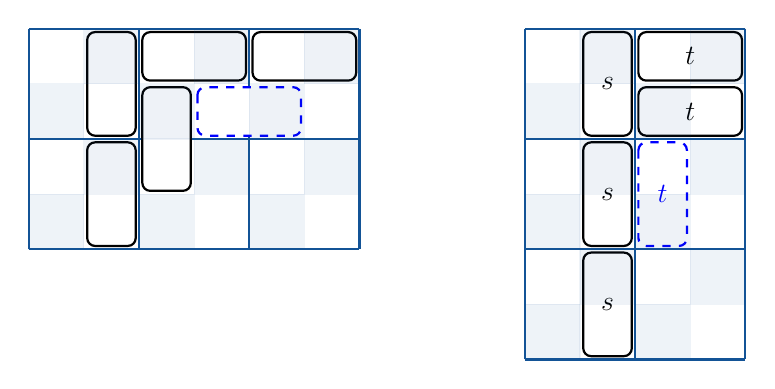
\begin{tikzpicture}[tableau, scale = .7]
          \gridLines{2}{3}
          \verticalDomino{1}{2}{}
          \horizontalDomino{1}{3}{}
          \horizontalDomino{1}{5}{}
          \verticalDomino{2}{3}{}
          \horizontalDominoMaybe{2}{4}{}
          \verticalDomino{3}{2}{}
          \fixedSquaresForGrid{2}{3}

          \gridLinesShift{3}{2}{9}
          \verticalDominoShift{1}{2}{s}{9}
          \horizontalDominoShift{1}{3}{t}{9}
          \horizontalDominoShift{2}{3}{t}{9}
          \verticalDominoShift{3}{2}{s}{9}
          \verticalDominoShift{5}{2}{s}{9}
          \verticalDominoMaybeShift{3}{3}{t}{9}
          \fixedSquaresForGridShift{3}{2}{9}
        \end{tikzpicture}
      \end{figure}
      \begin{figure}[H]
        % 1s 2s 3t 4t 5- 6+ 7+
        \centering
        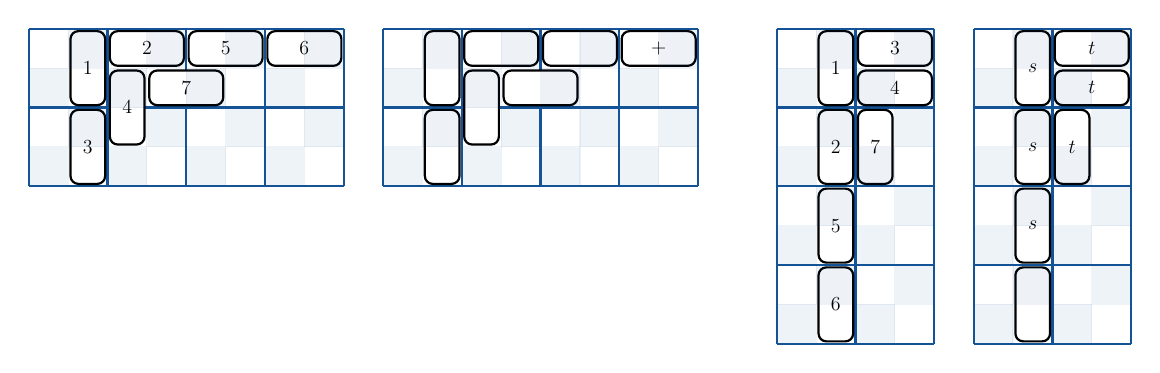
\begin{tikzpicture}[tableau, scale=.5]\gridLines{2}{4}\verticalDomino{1}{2}{1}\horizontalDomino{1}{3}{2}\verticalDomino{3}{2}{3}\verticalDomino{2}{3}{4}\horizontalDomino{1}{5}{5}\horizontalDomino{1}{7}{6}\horizontalDomino{2}{4}{7}\fixedSquaresForGrid{2}{4}\gridLinesShift{2}{4}{9}\verticalDominoShift{1}{2}{}{9}\horizontalDominoShift{1}{3}{}{9}\verticalDominoShift{3}{2}{}{9}\verticalDominoShift{2}{3}{}{9}\horizontalDominoShift{1}{5}{}{9}\horizontalDominoShift{1}{7}{+}{9}\horizontalDominoShift{2}{4}{}{9}\fixedSquaresForGridShift{2}{4}{9}\gridLinesShift{4}{2}{19}\verticalDominoShift{1}{2}{1}{19}\verticalDominoShift{3}{2}{2}{19}\horizontalDominoShift{1}{3}{3}{19}\horizontalDominoShift{2}{3}{4}{19}\verticalDominoShift{5}{2}{5}{19}\verticalDominoShift{7}{2}{6}{19}\verticalDominoShift{3}{3}{7}{19}\fixedSquaresForGridShift{4}{2}{19}\gridLinesShift{4}{2}{24}\verticalDominoShift{1}{2}{s}{24}\verticalDominoShift{3}{2}{s}{24}\horizontalDominoShift{1}{3}{t}{24}\horizontalDominoShift{2}{3}{t}{24}\verticalDominoShift{5}{2}{s}{24}\verticalDominoShift{7}{2}{}{24}\verticalDominoShift{3}{3}{t}{24}\fixedSquaresForGridShiftAlt{4}{2}{24}\end{tikzpicture}
      \end{figure}
    \end{itemize}
    \item Here the sign in the above row is $+$,
    the adjacent domino is vertical, and the unboxed cycle has at least two dominoes in it.
    So, we can't add here as a horizontal domino.
    However, we can add here as a vertical domino, contracting the unboxed cycle.
    First, if the pair domino is blank, we need to put the $+$ sign into the top of the cycle, which may result in a shape change.
    After that, we can add the new domino.
    Then we box up the adjacent domino and the domino which it is paired with.

    First, a simple example.
    \begin{figure}[H]
      \centering
      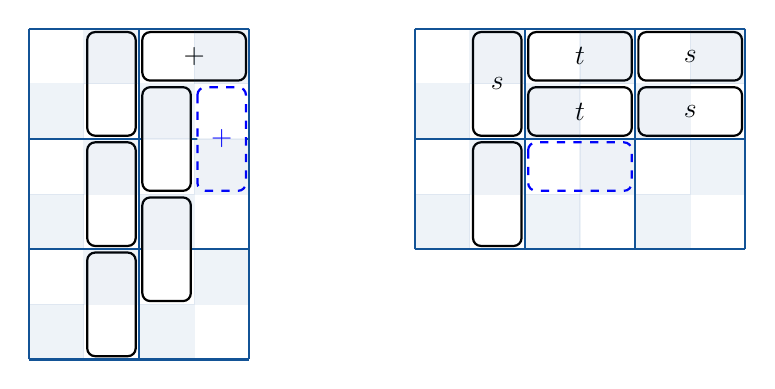
\begin{tikzpicture}[tableau, scale = .7]
        \gridLines{3}{2}
        \verticalDomino{1}{2}{}
        \horizontalDomino{1}{3}{+}
        \verticalDomino{2}{3}{}
        \verticalDominoMaybe{2}{4}{+}
        \verticalDomino{3}{2}{}
        \verticalDomino{4}{3}{}
        \verticalDomino{5}{2}{}
        \fixedSquaresForGrid{3}{2}

        \gridLinesShift{2}{3}{7}
        \verticalDominoShift{1}{2}{s}{7}
        \horizontalDominoShift{1}{3}{t}{7}
        \horizontalDominoShift{2}{3}{t}{7}
        \horizontalDominoShift{1}{5}{s}{7}
        \horizontalDominoShift{2}{5}{s}{7}
        \verticalDominoShift{3}{2}{}{7}
        \horizontalDominoMaybeShift{3}{3}{}{7}
        \fixedSquaresForGridShift{2}{3}{7}
      \end{tikzpicture}
    \end{figure}
    goes to
    \begin{figure}[H]
      \centering
      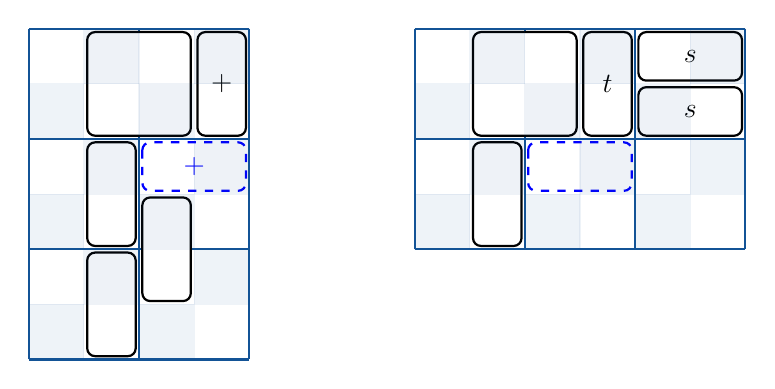
\begin{tikzpicture}[tableau, scale = .7]
        \gridLines{3}{2}
        \emptyBox{1}{2}
        \verticalDomino{1}{4}{+}
        \horizontalDominoMaybe{3}{3}{+}
        \verticalDomino{3}{2}{}
        \verticalDomino{4}{3}{}
        \verticalDomino{5}{2}{}
        \fixedSquaresForGrid{3}{2}

        \gridLinesShift{2}{3}{7}
        \emptyBoxShift{1}{2}{7}
        \verticalDominoShift{1}{4}{t}{7}
        \horizontalDominoShift{1}{5}{s}{7}
        \horizontalDominoShift{2}{5}{s}{7}
        \verticalDominoShift{3}{2}{}{7}
        \horizontalDominoMaybeShift{3}{3}{}{7}
        \fixedSquaresForGridShift{2}{3}{7}
      \end{tikzpicture}
    \end{figure}
    \begin{figure}[H]
      % 1s 2+ 3t 4t 5s 6s 7+
      \centering
      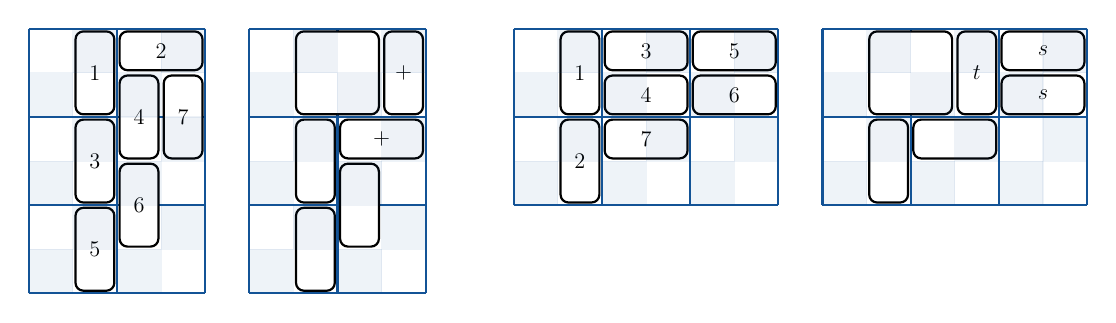
\begin{tikzpicture}[tableau, scale=.56]\gridLines{3}{2}\verticalDomino{1}{2}{1}\horizontalDomino{1}{3}{2}\verticalDomino{3}{2}{3}\verticalDomino{2}{3}{4}\verticalDomino{5}{2}{5}\verticalDomino{4}{3}{6}\verticalDomino{2}{4}{7}\fixedSquaresForGrid{3}{2}\gridLinesShift{3}{2}{5}\verticalDominoShift{1}{4}{+}{5}\verticalDominoShift{3}{2}{}{5}\verticalDominoShift{5}{2}{}{5}\verticalDominoShift{4}{3}{}{5}\horizontalDominoShift{3}{3}{+}{5}\emptyBoxShift{1}{2}{5}\fixedSquaresForGridShift{3}{2}{5}\gridLinesShift{2}{3}{11}\verticalDominoShift{1}{2}{1}{11}\verticalDominoShift{3}{2}{2}{11}\horizontalDominoShift{1}{3}{3}{11}\horizontalDominoShift{2}{3}{4}{11}\horizontalDominoShift{1}{5}{5}{11}\horizontalDominoShift{2}{5}{6}{11}\horizontalDominoShift{3}{3}{7}{11}\fixedSquaresForGridShift{2}{3}{11}\gridLinesShift{2}{3}{18}\verticalDominoShift{3}{2}{}{18}\verticalDominoShift{1}{4}{t}{18}\horizontalDominoShift{1}{5}{s}{18}\horizontalDominoShift{2}{5}{s}{18}\horizontalDominoShift{3}{3}{}{18}\emptyBoxShift{1}{2}{18}\fixedSquaresForGridShiftAlt{2}{3}{18}\end{tikzpicture}
    \end{figure}

    Next, an example with shape change.
    \begin{figure}[H]
      \centering
      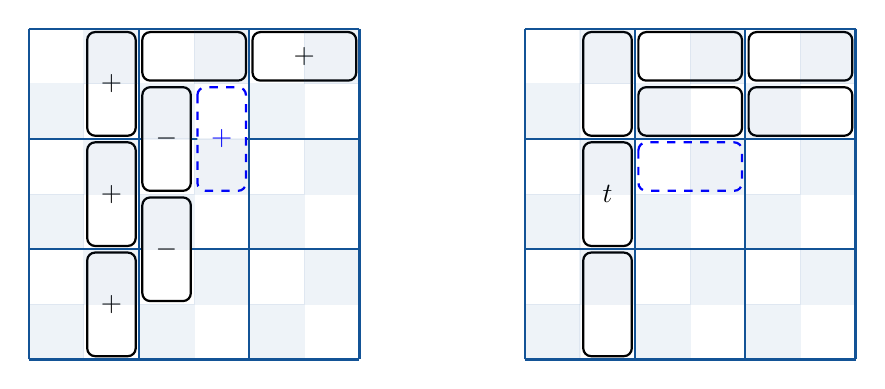
\begin{tikzpicture}[tableau, scale = .7]
        \gridLines{3}{3}
        \verticalDomino{1}{2}{+}
        \horizontalDomino{1}{3}{}
        \horizontalDomino{1}{5}{+}
        \verticalDomino{2}{3}{-}
        \verticalDominoMaybe{2}{4}{+}
        \verticalDomino{3}{2}{+}
        \verticalDomino{4}{3}{-}
        \verticalDomino{5}{2}{+}
        \fixedSquaresForGrid{3}{3}

        \gridLinesShift{3}{3}{9}
        \verticalDominoShift{1}{2}{}{9}
        \horizontalDominoShift{1}{3}{}{9}
        \horizontalDominoShift{2}{3}{}{9}
        \horizontalDominoShift{1}{5}{}{9}
        \horizontalDominoShift{2}{5}{}{9}
        \verticalDominoShift{3}{2}{t}{9}
        \verticalDominoShift{5}{2}{}{9}
        \horizontalDominoMaybeShift{3}{3}{}{9}
        \fixedSquaresForGridShift{3}{3}{9}
      \end{tikzpicture}
    \end{figure}
    \begin{figure}[H]
      % 1s 2+ 3_-4 5_-6 7+ 8+
      \centering
      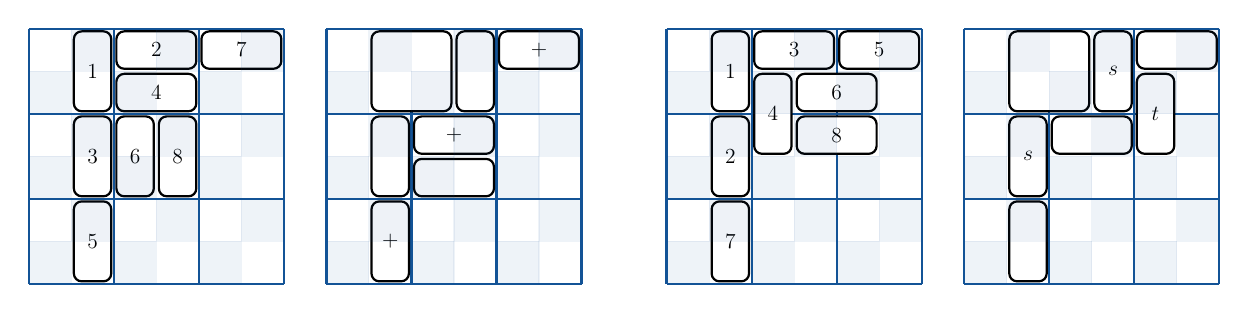
\begin{tikzpicture}[tableau, scale=.54]\gridLines{3}{3}\verticalDomino{1}{2}{1}\horizontalDomino{1}{3}{2}\verticalDomino{3}{2}{3}\horizontalDomino{2}{3}{4}\verticalDomino{5}{2}{5}\verticalDomino{3}{3}{6}\horizontalDomino{1}{5}{7}\verticalDomino{3}{4}{8}\fixedSquaresForGrid{3}{3}\gridLinesShift{3}{3}{7}\verticalDominoShift{1}{4}{}{7}\verticalDominoShift{3}{2}{}{7}\verticalDominoShift{5}{2}{+}{7}\horizontalDominoShift{4}{3}{}{7}\horizontalDominoShift{1}{5}{+}{7}\horizontalDominoShift{3}{3}{+}{7}\emptyBoxShift{1}{2}{7}\fixedSquaresForGridShift{3}{3}{7}\gridLinesShift{3}{3}{15}\verticalDominoShift{1}{2}{1}{15}\verticalDominoShift{3}{2}{2}{15}\horizontalDominoShift{1}{3}{3}{15}\verticalDominoShift{2}{3}{4}{15}\horizontalDominoShift{1}{5}{5}{15}\horizontalDominoShift{2}{4}{6}{15}\verticalDominoShift{5}{2}{7}{15}\horizontalDominoShift{3}{4}{8}{15}\fixedSquaresForGridShift{3}{3}{15}\gridLinesShift{3}{3}{22}\verticalDominoShift{3}{2}{s}{22}\verticalDominoShift{1}{4}{s}{22}\horizontalDominoShift{1}{5}{}{22}\verticalDominoShift{2}{5}{t}{22}\verticalDominoShift{5}{2}{}{22}\horizontalDominoShift{3}{3}{}{22}\emptyBoxShift{1}{2}{22}\fixedSquaresForGridShiftAlt{3}{3}{22}\end{tikzpicture}
    \end{figure}
    \item Here the sign in the above row is $+$,
    the adjacent domino is vertical, and the unboxed cycle consists solely of the adjacent domino.
    We may be able to add here.
    However, if we add here (as in the previous case), we'll end up with a horizontal domino with a $+$ sign in the $y + 1$ row.
    We need to see if that's possible, using the function \texttt{findRowToAddSignX()}.
    If not, we add at the row indicated by the return value of that function.

    If we can add here, we need to check first for a shape change from putting a $+$ sign in the cycle.
    Basically, we proceed as in the previous case.

    First, a simple example.
    \begin{figure}[H]
      \centering
      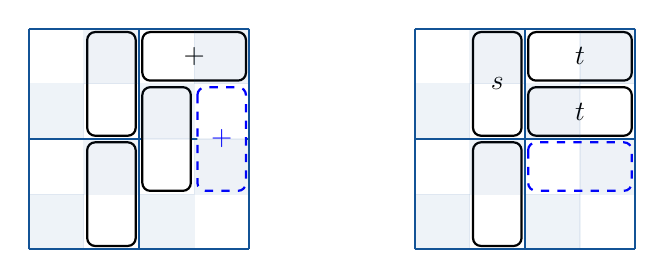
\begin{tikzpicture}[tableau, scale = .7]
        \gridLines{2}{2}
        \verticalDomino{1}{2}{}
        \horizontalDomino{1}{3}{+}
        \verticalDomino{2}{3}{}
        \verticalDominoMaybe{2}{4}{+}
        \verticalDomino{3}{2}{}
        \fixedSquaresForGrid{2}{2}

        \gridLinesShift{2}{2}{7}
        \verticalDominoShift{1}{2}{s}{7}
        \horizontalDominoShift{1}{3}{t}{7}
        \horizontalDominoShift{2}{3}{t}{7}
        \verticalDominoShift{3}{2}{}{7}
        \horizontalDominoMaybeShift{3}{3}{}{7}
        \fixedSquaresForGridShift{2}{2}{7}
      \end{tikzpicture}
    \end{figure}
    goes to
    \begin{figure}[H]
      \centering
      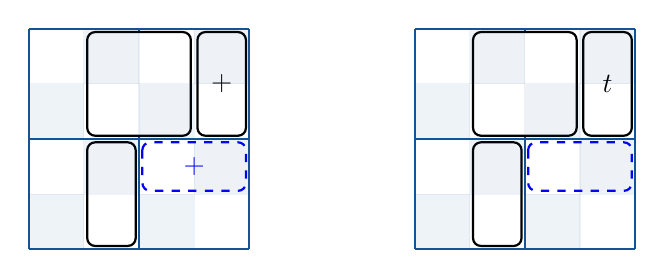
\begin{tikzpicture}[tableau, scale = .7]
        \gridLines{2}{2}
        \emptyBox{1}{2}
        \verticalDomino{1}{4}{+}
        \horizontalDominoMaybe{3}{3}{+}
        \verticalDomino{3}{2}{}
        \fixedSquaresForGrid{2}{2}

        \gridLinesShift{2}{2}{7}
        \emptyBoxShift{1}{2}{7}
        \verticalDominoShift{1}{4}{t}{7}
        \verticalDominoShift{3}{2}{}{7}
        \horizontalDominoMaybeShift{3}{3}{}{7}
        \fixedSquaresForGridShift{2}{2}{7}
      \end{tikzpicture}
    \end{figure}
    Next, an example with shape change.
    \begin{figure}[H]
      \centering
      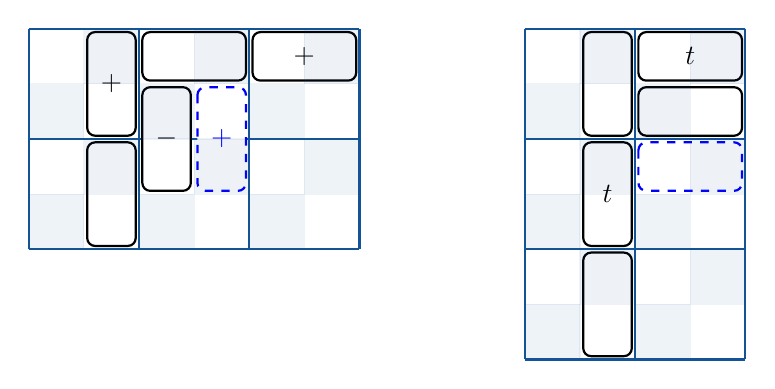
\begin{tikzpicture}[tableau, scale = .7]
        \gridLines{2}{3}
        \verticalDomino{1}{2}{+}
        \horizontalDomino{1}{3}{}
        \horizontalDomino{1}{5}{+}
        \verticalDomino{2}{3}{-}
        \verticalDominoMaybe{2}{4}{+}
        \verticalDomino{3}{2}{}
        \fixedSquaresForGrid{2}{3}

        \gridLinesShift{3}{2}{9}
        \verticalDominoShift{1}{2}{}{9}
        \horizontalDominoShift{1}{3}{t}{9}
        \horizontalDominoShift{2}{3}{}{9}
        \verticalDominoShift{3}{2}{t}{9}
        \verticalDominoShift{5}{2}{}{9}
        \horizontalDominoMaybeShift{3}{3}{}{9}
        \fixedSquaresForGridShift{3}{2}{9}
      \end{tikzpicture}
    \end{figure}
    \begin{figure}[H]
      % 1- 2+ 3s 4s 5+ 6+
      \centering
      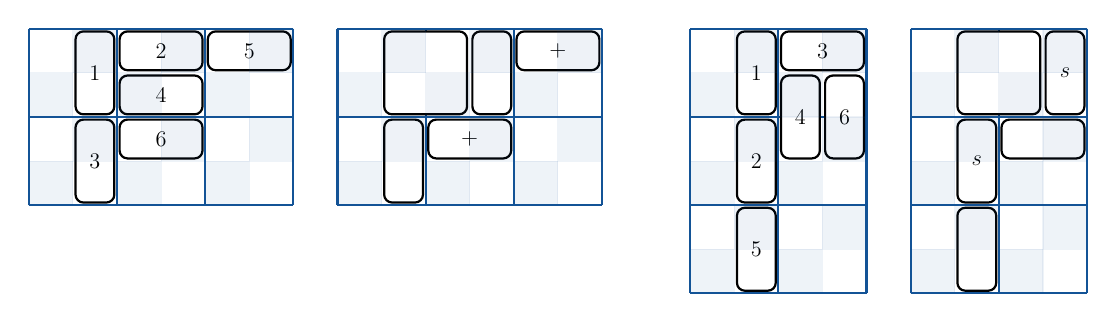
\begin{tikzpicture}[tableau, scale=.56]\gridLines{2}{3}\verticalDomino{1}{2}{1}\horizontalDomino{1}{3}{2}\verticalDomino{3}{2}{3}\horizontalDomino{2}{3}{4}\horizontalDomino{1}{5}{5}\horizontalDomino{3}{3}{6}\fixedSquaresForGrid{2}{3}\gridLinesShift{2}{3}{7}\verticalDominoShift{1}{4}{}{7}\verticalDominoShift{3}{2}{}{7}\horizontalDominoShift{1}{5}{+}{7}\horizontalDominoShift{3}{3}{+}{7}\emptyBoxShift{1}{2}{7}\fixedSquaresForGridShift{2}{3}{7}\gridLinesShift{3}{2}{15}\verticalDominoShift{1}{2}{1}{15}\verticalDominoShift{3}{2}{2}{15}\horizontalDominoShift{1}{3}{3}{15}\verticalDominoShift{2}{3}{4}{15}\verticalDominoShift{5}{2}{5}{15}\verticalDominoShift{2}{4}{6}{15}\fixedSquaresForGridShift{3}{2}{15}\gridLinesShift{3}{2}{20}\verticalDominoShift{3}{2}{s}{20}\verticalDominoShift{1}{4}{s}{20}\verticalDominoShift{5}{2}{}{20}\horizontalDominoShift{3}{3}{}{20}\emptyBoxShift{1}{2}{20}\fixedSquaresForGridShiftAlt{3}{2}{20}\end{tikzpicture}
    \end{figure}
  \end{itemize}
\end{document}
